%!TEX root = ../document.tex
\chapter{Lösungsansatz} \label{chp:Loesungsansatz}
In diesem Kapitel wird ein Verfahren zur Georeferenzierung von Twitter-Nutzern vorgestellt.
Die Fragestellungen aus Kapitel \ref{sec:fragestellung} werden, unter Berücksichtigung der Anforderungen aus Kapitel \ref{sec:Anforderungen}, beantwortet.  

Zunächst soll ein Überblick über die Funktion und den Ablauf des Verfahrens gegeben werden ohne detailliert auf die einzelnen Verfahrensschritte einzugehen.
Danach wird das Verfahen detaillierter betrachtet und die einzelnen Verfahrensschritte eingehender erläutert. 

	\section{Überblick} \label{sec:ueberblick} 
	\todo{evtl. allgemeine und diesen Teil nach unten ziehen wenn konkret auf Twitter eingegangen wird.} 
	Das erarbeitete Verfahren soll es ermöglichen Twitter-Nutzern eine Georeferenz zuzuordnen.
	Dabei sollen als Eingabe für die Georeferenzierung lediglich der Nutzer-Standort und die Nutzer-Zeitzone aus dem Profil eines Twitter-Nutzers verwendet werden.
	Als Ergebnis soll eine Georeferenz mit einem Konfidenzwert zurückgeliefert werden. 
	Dabei hat der Anwender die Möglichkeit, sowohl die Genauigkeit bezüglich der geografischen Position, als auch einen Schwellwert für die gewünschte Konfidenz anzugeben.
	In Abbildung \ref{img:georef} ist der generelle Ablauf dieser Georeferenzierung dargestellt. 
	\todo{Schema Darstellung Eingabe->Ausgabe  Sketchbook A1: Unterschrift Die Eingabe besteht aus dem Nutzer-Standort sowie der Nutzer-Zeitzone. 
	Als Rahmenbedingungen wird die gewünschte Hierarchie-Ebene sowie der Schwellwert für die Konfidenz angeben. 
	Als Ausgabe erhält man eine Georeferenz} 
	

	\begin{figure}[h!]
		\begin{center}
			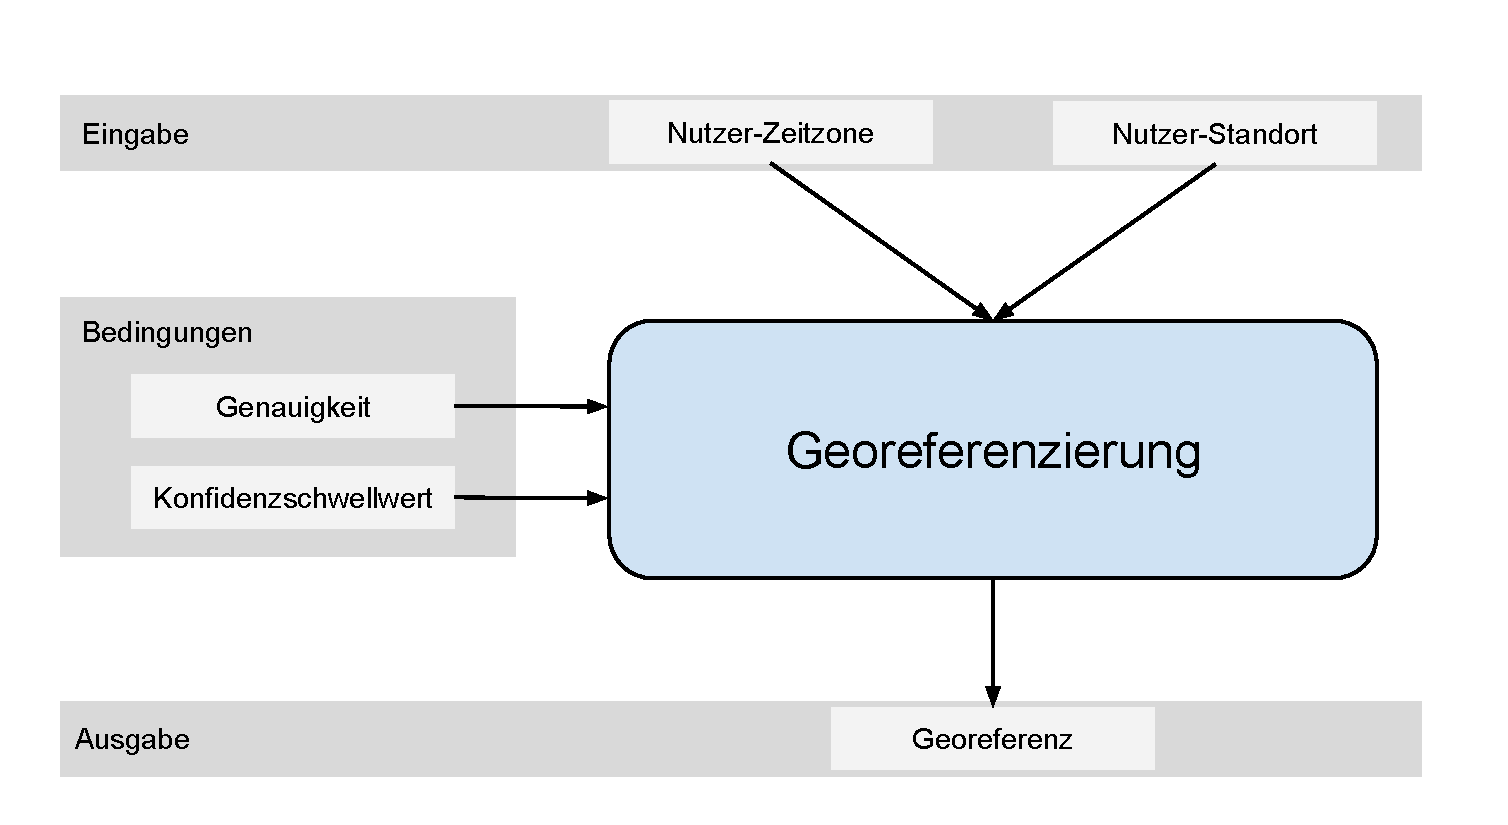
\includegraphics[scale=0.5]{A1.pdf}
			\caption{Ablauf Georeferenzierung}
			\label{img:georef}
		\end{center}
	\end{figure}	

	\todo{Neues Schema mit Objekt welchem mehrere geografische Indikatoren zugeordnet werden, Objekt beinhaltet Datensatz -> Georeferenzierung dieses Datensatzes} 
	Die Georeferenzierung nach dem Schema aus Abbildung \ref{A1} setzt voraus, dass aus den eingegebenen Indikatoren eine Georeferenz abgeleitet werden kann.
	Da es sich beim Nutzer-Standort und der Nutzer-Zeitzone um unmittelbare geografische Indikatoren handelt, lässt sich ein geografischer Bezug aus diesen Indikatoren ableiten.      
	Der Wert des Nutzer-Standortes kann vom Nutzer frei eingegeben werden.
	Es wird keinerlei Kontrolle oder Verifizierung durch Twitter durchgeführt.
	Wie in \ref{chp:Grundlagen} bereits analyisert wurde ist der Wert des Nutzer-Standortes nicht objektiv, nicht zuverlässig und nicht gesichert.
	Dies führt zu Problemen bei der Auswertung des Nutzer-Standortes.
	Um diesen Problemen zu begegnen soll aus einer umfangreichen Tweet-Datensammlung die Zuordnung der eingegebenen Indikatoren zu geografischen Positionen gelernt werden.
	Diese gelernten Zuordnungen sollen in einer Datenbasis gespeichert werden.
	Die Datenbasis wird Georeferenz-Basis genannt.
	
	Zur Erstellung der Georeferenz-Basis werden zunächst einige Schritte zur Vorverarbeitung der Indikatoren durchgeführt.
	Zusätzlich wird, die in jedem Tweet anegegebene Georeferenz, verarbeitet.
	In der Georeferenz-Basis werden nun die so erstellen Indikator-Werte mit den entsprechenden Georeferenzen gespeichert.
	Dadurch entsteht ein Wörterbuch mit Indikatoren und zugehörigen geografischen Objekten, die Georeferenz-Basis.
	Der gesamte Ablauf zur Erstellung der Georeferenz-Basis wird in Abbildung \ref{A2} dargestellt.

	Bei der Georeferenzierung werden die Indikatoren zunächst derselben Vorverarbeitung wie beim einlernen unterzogen.
	Die Vorverarbeitungsschritte sind somit generisch, da sie sowohl vor dem erzeugen der Georeferenz-Basis als auch vor der eigentlichen Georeferenzierung durchgeführt werden.
	Nach der Vorverarbeitung werden die Indikatoren in der Georeferenz-Basis nachgeschlagen und es kann eine Georeferenz zugeordnet werden.
	Der Ablauf der Georeferenzierung wird in Abbildung \ref{A3} dargestellt. 

	\todo{Ablaufplan A1, A2, A3} 

		In den folgenden Kapiteln soll nun genauer auf die einzelnen Teile des Verfahrens eingegangen werden. 
		Das Verfahren wird dabei in zwei Teilen behandelt.

	\paragraph{Einlernen der Georeferenz-Basis}  

		In diesem Teil wird erklärt wie mit Hilfe einer Tweet-Sammlung die Georeferenz-Basis durch ein Lern-Verfahren erstellt wird.
		Zunächst werden die verwendeten Indikatoren untersucht.
		Basierend auf diesen Erkenntnissen wird ein erster Ansatz zur Umsetzung eines Lern-Verfahrens vorgestellt.
		Mit Hilfe dieses ersten Ansatzes wird das Verfahren sukzessive weiterentwickelt bis die angestrebten Anforderungen erfüllt werden können.  
		Im Zuge dessen werden die generischen Vorverarbeitungsschritte zur Verarbeitung der Indikatoren entwickelt und erläutert.
		Auch die Vorverearbeitung, der in jedem Tweet angegeben geografischen Koordinaten, soll hier behandelt werden.
		Danach soll der gesamte Ablauf des Einlernens noch einmal dargestellt und kurz erklärt werden um einen Gesamtüberblick zu liefern.
	
	\paragraph{Georeferenzierung} 

		Die Vorverarbeitungsschritte der Indikatoren wird in diesem Teil nur angeschnitten, da diese bereits im ersten Teil genau erläutert werden. 
		Die Georeferenzierung besteht im Grunde lediglich aus einer Abfrage an die Georeferenz-Basis und die Auswertung der Ergebnisse.
		Bei der Auswertung wird insbesondere auf die konkrete Berechnung der Konfidenzen eingegangen.
		Am Ende dieses Teils steht das Ergebnis der Georeferenzierung. 


	\section{Generelle Struktur einer Datenbasis zum nachschlagen geografischer Indikatoren}

		In diesem Kapitel soll eine generelle Struktur angegeben werden, welche die minimalen Anforderungen einer Georeferenzierung erfüllen kann.
		Danach wird das Schema und die nötigen Informationen welche die Datenbasis beinhaltet genauer betrachtet.
		
		% Danach wird an einem Beispiel motiviert wie es möglich ist eine solche Datenbasis automatisch einlernen zu lassen und wieso dies sinnvoll ist.
		% Zum einlernen der Datenbasis wird ein allgemeines Schema vorgestellt.
		% Im Zuge dessen werden die minimalen Anforderungen an die Lern-Daten zunächst allgemein erläutert, um dann auf die genutzten Lern-Daten aus dem Twitter-Netzwerk einzugehen.
		% Danach wird erklärt wie mit Hilfe von Häufigkeitswerten Konfidenzen berechnet werden können. 
		% Des weiteren wird die Einbeziehung geografischer Hierarchien eingehend betrachtet, dabei wird erklärt wie diese genutzt werden können um die geografische Genauigkeit zu bestimmen.  

		Nach Abbildung \ref{img:allgA1} wird durch die Georeferenzierung einer Menge geografischer Indikatoren eine Georeferenz zugewiesen.
		In der einfachsten Variante wird lediglich ein einziger geografischer Indikator an die Georeferenzierung übergeben und genau eine Georeferenz zurückgegeben.
		Die Georeferenzierung muss also zu einem gegebenen geografischen Indikator eine Georeferenz bestimmen können.
		Dies führt zu einer ersten einfachen Struktur für die Datenbasis.	

		\subsection*{Eine erste einfache Struktur der Datenbasis} 

			Es wird angenommen der geografische Indikator stellt immer ein eindeutiges Toponym dar.
			Des weiteren sind alle möglichen Toponyme sowie eine zugehörige Georeferenz bekannt. 
			Die Georeferenz liegt als Adresse mit Straße, Hausnummer, Postleitzahl und Ortsname vor.

			Jedem möglichen Toponym, welches im gegebenen geografischen Indikator vorkommen kann, soll eine Georeferenz zugeordnet werden können. 
			Daraus ergibt sich die Anforderung, dass die Datenbasis eine Menge von Datensätzen beinhalten muss, die jeweils aus einem Toponym und einer Georeferenz bestehen.
			Dieser Aufbau entspricht einer Art Wörterbuch in dem Informationen zu einem gegebenen Referenzwert nachgeschlagen werden können.
			Im vorliegenden Fall kann also zu einem Toponym die enstprechende Georeferenz nachgeschlagen werden.
			Die Referenzwerte stellen dabei mögliche Werte für die Indikatoren dar. 
			In Abbildung \ref{tab:simpleStruktur} ist ein Beispiel für eine sehr simplen Struktur dargestellt.

			\begin{table}[htpb]
					\caption{Erste einfache Struktur für eine Datenbasis zur Georeferenzierung} 
					\centering
					\begin{tabular}{|c|c|}
						\hline
						Referenzwert & Georeferenz \\
						\hline\hline
						Zoo-Karlsruhe & Ettlinger Straße 6 - 76137 Karlsruhe \\
						\hline
						ZKM & Lorenzstraße 19 D - 76135 Karlsruhe \\
						\hline
						Elbphilharmonie & Dammtorwall 46 - 20355 Hamburg \\
						\hline
					\end{tabular}
					\label{tab:simpleStruktur} 
			\end{table} 

			Wird eine Abfrage auf die Datenbasis mit den Indikatoren '"Zoo-Karlsruhe'", '"ZKM'" oder "'Elbphilharmonie'" durchgeführt, kann nun eine Georeferenz zurückgeliefert werden.
			Diese simple Struktur reicht grundsätzlich aus um eine Georeferenzierungen durchführen zu können.
			In dem angeführten Beispiel ist die Menge der möglichen Toponyme sehr begrenzt, aber diese kann beliebig erweitert werden.
			Damit können sehr mächtige Datenbanken erstellt werden.

			Es sollen nun der Referenzwert und die Georeferenz genauer betrachtet werden.

			\paragraph{Form der Georeferenz}

				Die Form in der die Georeferenz angegeben wird ist abhängig von der Anwendung. 
				Im Beispiel \ref{tab:simpleStruktur} wurden Adressen verwendet. 
				Dazu muss das angegebene Toponym oder die Zeichenkette jedoch eine Adresse besitzen. 
				Ein See in der Wildnis Alaskas wird keine solche Adresse aufweisen.
				Aber auch die geografische Position einer Stadt oder eines Landes kann nicht durch eine Adresse beschrieben werden. 
				Die Form in der die Georeferenz angegeben wird kommt auf den jeweiligen Anwendungsfall an.
				Denkbar sind hier unter anderem:

				\begin{itemize}
				  	 \item geografische Koordinaten
				  	 \item vollständige Adressen
				  	 \item Länder
				  	 \item Städte
				  	 \item adminsitrative Verwaltungsgebiete 
				  	 \item Zeitzonen
				  	 \item Straßenname und eine Kilometerbezeichnung
				  \end{itemize}  

				  Grundsätzlich sind alle Formen, welche eine direkte oder indirekte Georeferenz darstellen, denkbar.
				  Wichtig ist nur, dass die Angabe der Georeferenz in einer Form erfolgt welche für die gegebene Anwendung ausreichend genau ist.

				  Für den Straßenverkehr ist eine Angabe einer Adresse ausreichend.
				  Für Wanderungen in unerschlossenen Gebieten hingegen sind geografische Koordinaten notwendig. 

			\paragraph{Form der Referenzwerte}

				Der Referenzwert ergibt sich aus den möglichen Werten der Indikatoren.
				Die Indikatoren sind dabei zumeist Zeichenketten.
				Abhängig vom Indikator können diese Zeichenketten verschiedene Informationen enthalten.
				Im obigen Beispiel sind die Referenzwerte Toponyme.
				Toponyme sind Namen für geografische Objekte, es kann ihnen also unmittelbar ein geografische Objekt zugeordnet werden.
				Es muss sich dabei aber nicht um Toponyme handeln.
				Geografische Indikatoren, und damit auch die Referenzwerte, können auch mittelbar mit einem geografischen Objekt in Verbindug gebracht werden.
				Unbrauchbar sind Werte welche weder mittelbar noch unmittelbar mit einem geografischen Objekt in Verbindung gebracht werden können.
				Diese Werte stellen keine geografischen Indikatoren dar.

	\section{Geografische Indikatoren} 

		Geografische Indikatoren sind diejenigen Indikatoren welche einen geografischen Bezug aufweisen.
		Es sind also genau die Werte eines Datensatzes, welche in irgendeiner Weise mit einem geografischen Objekt in Verbindung gebracht werden können.
		Geografische Indikatoren lassen sich in unmittelbare geografische Indikatoren und mittelbare geografische Indikatoren aufteilen. 
		In diesem Abschnitt soll sowohl auf die unmittelbaren wie auch die mittelbaren geografischen Indikatoren eingegangen werden.

			\subsection{Unmittelbare geografische Indikatoren} \label{subsec:unmittelbareGeografischeIndikatoren} 

				Der in einem unmittelbaren geografischen Indikator angegebene Wert beschreibt direkt eine geografische Position oder eine geografische Region.	
				Einem unmittelbaren geografischen Indikator kann durch die in ihm enthaltene Information direkt eine Georeferenz auf ein geografisches Objekt zugewiesen werden. 

				Im Beispiel in Tabelle \ref{tab:simpleStruktur} wurden unmittelbare geografische Indikatoren verwendet.
				Die Referenzwerte entsprechen Toponymen, sie sind Namen für geografische Objekt. 
				Ihnen kann also unmittelbar ein geografisches Objekt zugeordnet werden.

				Ein weiteres Beispiel für einen unmittelbaren geografischen Indikator sind Zeitzonen.

				Bei der Zeitzone handelt es sich um einen geografischen Indikator der eine geografische Region beschreibt. 
				Die zugehörige Georeferenz für eine Zeitzone könnten die Länder sein welche die Zeitzone umfasst. 
				Aber auch die Kontinente oder Städte welche in dieser Zeitzone liegen könnten, je nach Anwendugsfall, von Interesse sein.


			\subsection{Mittelbare geografische Indikatoren} 

				Der Indikator muss aber nicht unmittelbar einer Georeferenz zuzuordnen sein.
				Dies ist genau dann der Fall, wenn der in eiem geografischen Indikator angegebene Wert in erster Linie nicht einem geografischen Objekt zugeordnet werden kann.
				
				Die Möglichkeiten was einen mittelbaren geografischen Indikator darstellen kann sind nahezu unbegrenzt. 
				An einem Beispiel soll ein gezeigt werden was einen mittelbaren geografischen Indikator ausmacht.
				
				\paragraph{Beispiel eines mittelbaren geografischen Indikators} 

				Es liegen drei Begriffe vor.
				\begin{enumerate}
				 	\item Äbierra
				 	\item Grumbeer
				 	\item Tüfte 
				 \end{enumerate} 

				Nach einer kurzen Recherche kann festgestellt werden, dass es sich bei allen drei Begriffen um Kartoffeln handelt.
				Die Information die hinter jedem dieser Begriffe steckt ist also die Bezeichnung eines Gemüses.
				Die Begriffe bezeichnen also insbesondere kein geografisches Objekt und sind somit keine unmittelbaren geografischen Indikatoren.
				Jede dieser Bezeichnungen stammt aber aus unterschiedlichen Regionen Deutschlands, denn es handelt sich um dialektiche Begriffe.
				Durch ihre geografisch begrenzte Verwendung können sie damit einer geografischen Region zugeordnet werden.
				Durch die Verwendung eines dieser Worte kann also auf eine Region Deutschlands geschlossen werden.
				Dadurch kann jedem Begriff eine Georeferenz zugewiesen werden.

				Mit folgender Datenbasis kann eine Georeferenzierung der obigen Begriffe durchgeführt werden:

				\begin{table}[htpb]
					\caption{Kartoffeln in verschiedenen Dialekten} 
					\centering
					\begin{tabular}{|c|c|}
						\hline
						Referenzwert & Georeferenz \\
						\hline\hline
						Äbbiera & Württemberg \\
						\hline
						Grumbeer & Pfalz \\
						\hline
						Tüfte & Norddeutschland \\
						\hline
					\end{tabular}
					\label{tab:dialekt} 
				\end{table} 

				In diesem Beispiel wurde die Zuordnung zu einem geografischen Objekt über die Verwendung der Begriffe in bestimmten Regionen ermöglicht.
				Aber auch andere Informationen können dazu dienen einem Indikator eine Georeferenz zuzuordnen.
				Es kommt grundsätzlich nicht darauf an was genau mit dem Begriff bezeichnet wird. 
				Lediglich die geografisch begrenzte Verwendung kann hier als Hinweis auf eine Georeferenz dienen. 

				Ein solcher geografischer Indikator wird als '"mittelbar geografischer Indikator'" bezeichnet. 

	\section{Der Nutzer-Standort eines Twitter-Nutzers als geografischer Indikator} \label{sec:nutzerStandort} 

				Grundsätzlich sind alle Daten, die zu einem Twitter-Nutzer verfügbar sind potenzielle geografische Indikatoren.
				Es gibt allerdings Indikatoren, welche sich aufgrund der Intention des Wertes besonders gut als geografische Indikatoren eignen.

				Dies trifft insbesondere auf den Nutzer-Standort zu.
				Dieser Eintrag wird vom Nutzer abgefragt mit der Intention eine geografische Angabe zu machen. 
				Der Nutzer-Standort kann vom Nutzer frei eingegeben werden und wird keinerlei Verarbeitung unterzogen.
				\todo{Bild Nutzer-Stadnort Eingabe} 

				Diese Eigenschaft hat weitreichende Folgen für die Nutzung des Nutzer-Standortes als geografischer Indikator und sollen nun untersucht werden.

			\subsection{Eigenschaften des Nutzer-Standortes} 

				Der Nutzer-Standort kann frei eingegeben werden und unterliegt, außer einer Längenbegrenzung von 30 Zeichen, keinerlei Restriktionen. 
				Das Feld wird von Twitter als '"Standort'" bezeichnet und kann vom Nutzer in den Profileinstellungen eingegeben werden. 
				Dies legt für den Nutzer Nahe einen Wert einzugeben, der einen geografischen Bezug aufweist.
				Die Werte müssen allerdings keinen geografischen Bezug aufweisen.

				\subsubsection{Weißt der Nutzer-Standort einen geografischen Bezug auf?} 
					
					Nach Hecht et al. haben in \cite{Hecht2011} den Nutzer-Standort eingehend untersucht und sind zu folgendem Ergebnis gekommen:
					Wenn der Nutzer überhaupt einen Standort angegegeben konnte in 80\% Prozent der Fälle ein geografischer Bezug nachgewiesen werden.
					In den restlichen 20\% der Fälle konnte im Nutzer-Standort kein geografischer Bezug nachgewiesen werden. 
					Die Untersuchung wurde manuell vorgenommen und es durften alle zur Verfügung stehenden Mittel zur Analyse der Daten verwendet werden. 
					Hecht et al. haben deshalb ausschließlich Daten untersucht die nachweislich aus den USA stammten. 

					Es kann hier also festgehalten werden, dass 80\% der Nutzer-Standorte als geografischer Indikator verwendet werden können.
					Es muss bechtet werden, dass nur Daten aus den USA betrachtet wurden.

					Im Rahmen der vorliegenden Arbeit wurde der Nutzer Standort von 1000 Twitter-Nutzern ebenfalls manuell untersucht. \footnote{siehe \ref{chp:AppendixA} }  
					Dabei wurde keinerlei Einschränkung zur Herkunft gemacht.
					Um zu prüfen ob ein geografischer Bezug vorliegt wurden Ortsverzeichnisse von Google-Maps und Geonames.org verwendet.
					Diese lassen es zu auch in dem Nutzer unbekannten Sprachen und Alphabeten zu suchen.
					Es konnte dabei in XYZ\% der Fälle ein geografischer Bezug nachgewiesen werden. 
					%Bei der Untersuchung noch darauf eingehen ob die manuelle Lokalsieirung mit dem geog. Koordinaten übereingestimmt hat

					In den restlichen XYZ\% der fälle konnte kein geografischer Bezug mit Hilfe der Datenbanken nachgewiesen werden. 
					Dies bedeutet nicht, dass grundsätzlich kein geografischer Bezug vorhanden ist. 
					Es konnte lediglich anhand der genutzten Quellen kein geografischer Bezug hergeleitet werden.

					Der Nutzer-Standort kann also in vielen Fällen einen Hinweis auf die Herkunft des Twitter-Nutzers geben.

				\subsubsection{Genauigkeit der geografischen Angaben}

					In 80\% der Fälle kann bei einer Angabe des Nutzer-Standortes davon ausgegangen werden, dass dieser geografischen Bezug hat.
					Wiederum aufgrund dessen, dass der Nutzer beliebige Eingaben machen kann, ist nicht sicher wie genau ein solcher geografischer Bezug ist. 
					
					Hecht et al. analyiserten ihre Daten auch darauf wie genau die Nutzer ihren Standort angeben.
					Dabei ist wiederum zu beachten, dass die Daten aus den USA stammten und deshalb die geografischen Verwatungsebenen der USA zugrunde gelegt wurden.
					Zusätzlich wurden hier auch 
					Dabei wurden folgende Werte festgestellt:

					\begin{itemize}
					 	\item 64\% Stadt 
					 	\item 20\% Staat (Adminstrationsebne erster Ordnung)
					 	\item ca. 8\% Intrastate (Adminstrationsebene zweiter Ordnung)
					 	\item ca. 5\% Land
					 \end{itemize} 

					 Die restlichen 13\% entfallen auf Interstate Regionen, Nachbarschaften und konkrete Adressen. 
					 Interstate Regionen sind Regionen die sich über mehrere Staaten hinwegziehen. 
					 Beispiele für Interstate Regionen sind '"Central United States"' oder '"West-Coast"'.
					 Nachbarschaften(Neighbourhoods) sind oft Stadtteile wie '"Harlem"' oder '"Bronx"' in New York.

					 In den eigenen Untersuchungen sind folgende Werte festgestellt worden:

					\begin{itemize}
					 	\item xyz\% Stadt 
					 	\item zz\% Adminstrationsebene erster Ordnung
					 	\item tt\% Adminstrationsebene zweiter Ordnung
					 	\item uu\% Land
					 \end{itemize} 

					Es hier gefolgert werden, dass selbst wenn ein geografischer Bezug besteht, nicht mit Sicherheit bestimmt werden kann wie genau dieser ist.

				\subsubsection{Partieller geografischer Bezug des Nutzer-Standortes}

					In einigen der Einträge konnte festgestellt werden, dass nur Teile der Einträge geografischen Bezug haben. 
					Oft wollen die Nutzer noch weitere Informationen geben, diese haben oft keinen Nutzen für eine Georeferenzierung. 
					In der folgenden Liste sind einige Einträge von Nutzer-Standorten aufgelistet. 

					\begin{enumerate}
						\item 11th Dimension | California
						\item between here and there - Miami
					\end{enumerate}

					Im ersten Fall kann für Kalifornien ein geografischer Bezug festgestellt werden.
					11th Dimension hat hier offensichtlich keinen geografischen Bezug.
					Im zweiten Fall ist die Aussage "'between here and there"' nicht zu gebrauchen, Miami kann jedoch als Bezug zur Stadt Miami in Florida, USA gebracht werden.
					
					Es können also auch nur Teile des Nutzer-Stadorts für eine Georeferenzierung von Nutzen sein.


				\subsubsection{Mehrere wiedersprüchliche geografische Bezüge} 

					Es existieren auch Einträge für Nutzer-Standorte welche mehrere Wiedersprüchliche Angaben machen.
					Das bedeutet es werden zwei oder mehr Werte mit geografischem Bezug angegegeben.

					Auch hier sollen einige Beispiele genannt werden:

					\begin{itemize}
						\item Bolton\\/Leigh
						\item Liverpool\\/London
						\item  Balikesir \\/ Izmir	
					\end{itemize}							
						
					In diesen Beispielen sind jeweils zwei Städte angegeben, Bolton und Leigh liegen 14km auseinander.
					Liverpool und London trennen ca. 350km.
					Balikesir und Izmir ca. 180km.

					Es kann nun spekuliert werden wieso der Nutzer zwei Städte angibt.
					Ist er in einer Stadt aufgewachsen und lebt momentan in der anderen?
					Pendelt er zwischen den Städten um zu arbeiten?

					Wie dem auch sei, es kann nicht eindeutig entschieden werden in welcher Stadt sich der Nutzer aufhält.
					

				\subsubsection{Fazit}

					Ist ein geografischer Bezug des Nutzer-Standortes nachzuweisen, handelt es sich bei dem Eintrag in den meisten Fällen um ein Toponym.
					Es wurden 100 Tweets untersucht und es wurden diesen Manuell Georeferenzen aus einem Ortsverzeichnis zugewiesen werden.
					Dadurch konnte gezeigt werden, dass ca. xyz\% der Nutzer-Standorte mit einem geografischen Bezug auf Toponyme zurückzuführen sind.
					Es ergab sich kein signifikanter Unterschied zu den Untersuchugen von Hecht et al..

					Zusammenfassend kann gesagt werden, dass der Nutzer-Standort häufig einen geografischen Bezug aufweist und es sich in diesen Fällen um Toponyme handelt.
					Aufgrund der völlig freien Eingabe durch den Nutzer ergeben sich bei der Auswertung der Nutzer-Standorte jedoch einige Probleme. 



				So haben beispielsweise "'kcmo--call da popo"' oder "'Bieberville, California"' geografischen Bezug.
				Auch nach den Untersuchungen im Zuge dieser Arbeit konnte festgestellt werden das ca. xyz Prozent der eingegebenen Werte tatsächlich ein Toponym darstellen und die Annahme somit korrekt ist. \footnote{
				Hecht et al. haben nur Nutzer-Standorte in englischer Sprache untersucht, wohingegen in den selbst durchgefürten Untersuchungen keine Einschränkung bezüglich der Sprache besteht} 

				% Hier sollen die grundsätzlichen Eigenschaften betrachtet werden. Darauf hinauslaufend, das oft Toponyme verwendet werden (Hecht Geschichten) und das aber auch mittelbare geog. Indikatoren auftreteten können. 
				% Im nächsten Abschnitt (Probleme bei der Verwendung unkontrollierte Toponyme) soll dann auf die Probleme der Toponyme und mittelbar geografischen Indikatoren eingegangen werden. (Doppel- und Mehrdeutigkeiten etc. pp. hier zusätzlichen Indikator Zeit-Zone einführen)
				% section Allgemeines Lernverfahren für geografische Ind. Mit den Problemen der Toponyme, dem potenziellen auftreten von mittelbar geog. Ind. soll dann das Lernverfahren begründet werden.
				% Beim Lernverfahren soll zunächst allgemein erklärt werden was geschieht -> Häufigkeitswerte danach geografische Hierarchie. (EInfach einführen und erklären was es tut!!!!!) 
				% section Vorverarbeitungsschritte bei der Verwendung des Nutzer-Standortes.

			\section{Probleme bei der Verwendung von Toponymen als geografische Indikatoren}

				Wie in Abschnitt 


				\subsection{Doppel- und Mehrdeutigkeiten} 

						Doppel- und Mehrdeutigkeiten können sowohl ausgehend von der Georeferenz, als auch ausgehend vom Referenzwert auftreten.

						\paragraph{Zu einem Referenzwert können mehrere Georeferenzen existieren}

							Am Beispiel von Toponymen soll dieser Sachverhalt erklärt werden.
							Es gibt beispielsweise zahlreiche Städte-Namen, die in mehreren Ländern verwendet werden.
							Ein gutes Beispiel hierfür sind US Städte. 
							Da die USA ein Einwanderungsland ist, übernahmen viele Einwanderer bei der Gründung neuer Städte die Namen aus der alten Heimat. 
							So finden sich in den USA zahlreiche Städte deren Namen exakt den deutschen Städtenamen entsprechen. 
							In Tabelle \ref{tab:usCitiesGemanNames} sind einige Städte-Namen und die Vorkommen in den USA aufgelistet.
							
							\begin{table}[htpb]
								\caption{Häufige deutsche Städtenamen in den USA} 
								\centering
								\begin{tabular}{|c|c|}
									\hline
									Name & Anzahl in den USA \\
									\hline\hline
									Hannover & 40 \\
									\hline
									Berlin & 39 \\
									\hline
									Hamburg & 30 \\
									\hline
								\end{tabular}
								\label{tab:usCitiesGermanNames} 
							\end{table}


							Soll nun eine Datenbasis angelegt werden, welche einem Stadt-Namen einen Staat zuweist hätte diese Tabelle für Hannover 40 Einträge mit dem Staat USA und einen für Deutschland.
							Als Ergebnis der Georeferenzierung würde 40 mal USA und ein mal Deutschland zurückgegeben werden. 
							Die Anzahl der Einträge hat dabei keinerlei Aussage über die Wahrscheinlichekit welches Hannover gemeint ist.

							Aber auch mittelbare geografische Indikatoren können von dieser Art der Mehrdeutigkeit betroffen sein.
							Beispielsweise wird Grumbeere sowohl in der Pfalz als auch in Württemberg als Bezeichnung für Kartoffeln verwendet.

							Die hier beschriebene Mehrdeutigkeit kann als 1-zu-N Beziehung zwischen Referenzwerten und Georeferenz betrachtet werden.
							Diese Mehrdeutigkeit stellt ein Problem bei der Georeferenzierung dar.
							Es kann keine eindeutige Entscheidung getroffen werden welche Georeferenz dem Ort zugewiesen werden soll. 
							\todo{Lösung über Konfidenzen} 

						\paragraph{Zu einer Georeferenz können mehrere Referenzwerte existieren}

							Es existieren sehr umfangreiche Datenbasen um Toponymen eine Georeferenz zuzuweisen. 
							Die Datenbank von geonames.org beinhaltet beispielsweise rund 8,9 Millionen Toponyme und zugehörige Georeferenzen.
							Zusätzlich sind weitere rund 8 Millionen alternative Toponyme hinterlegt.
							Allerdings ist es aufgrund der Vielfalt der Toponyme nahezu unmöglich eine vollständige Datenbank zu erstellen.

							Beispielsweise werden in Wikipedia für die Stadt Detroit, im US-Bundesstaat Michigan, folgende Spitznamen angegeben:
							\begin{itemize}
								\item The Motor City
								\item Motown
								\item Hockeytown
								\item The D. 
							\end{itemize}

							Die ersten zwei dürften weltweit einen Gewissen Bekanntheitsgrad haben. 
							Hockeytown, Rock City und The D dürften allerdings weniger bekannt sein.  
							
							Auch besteht die Möglichkeit, dass Spitznamen für Städte existieren die kaum über die Grenzen eines Landes, oder sogar der Stadt selbst bekannt sind. 
							Neben diesen Beispielen sind aber auch Toponyme denkbar die einen bestimmten Landstrich oder eine landschaftliche Besonderheit beschreiben.
							Beispielsweise beschreibt '"An der Förde'" eine geografische Region an der Ostsee, meist ist damit die Kieler Förde und dessen Umgebung gemeint. 
							Diese geografischen Bezeichnungen sind unter Umständen nur in speziellen Datenbanken zu finden und können so nur schlecht aufgelöst werden. 

							Es ist schwer, wenn nicht sogar unmöglich, das Wissen über geografische Objekte und deren zugehörige Toponyme vollständig zu erfassen.
							Geonames.org beinhaltet trotz der immensen Vielfalt an Toponymen die oben angeführten Stadtspitznamen von Detroit nicht.



							Dies ist grundsätzlich auf alle geografischen Objekte übertragbar.
							Zu jedem geografischen Objekt existieren potenziell meherere gültige Toponyme.
							Diese Mehrdeutigkeit kann als 1-zu-N Beziehung zwischen Georeferenz und Referenzwerten angesehen werden.
							Das Problem bei dieser Art der Mehrdeutgkeit ist, dass es praktisch nicht möglich ist alle Toponyme für alle geografischen Objekte zu sammeln. 
							Eine Teillösung wäre es Informationen aus verschiedenen Datenbanken zu integrieren um soviele Referenzwerte wie möglich zu vereinen.
							Hier wurden nur unmittelbare geografische Indikatoren betrachtet.

							Aber diese Mehrdeutigkeiten gelten insbesondere auch für mittelbare geografische Indikatoren.
							Am Beispiel der dialektischen Begriffe kann dies gut verdeutlicht werden.
							Lässt man beispielsweise neben den Bezeichnugen für Kartoffeln noch andere dialektische Worte zu können diese Mehrdeutigkeiten enstehen.
							Im württembergischen steht Guatsle für Bonbon. 
							Damit wird Württemberg sowohl Guatsle als auch Äbbiera zugeordnet.

							\todo{Lösung über Lernen beim lernen auch unbekannte mittelbare geografische Indikatoren einbeziehen über unbekannte Eingabe Beispiel Briefe.} 

				\subsection{Fazit}

					Es existieren sehr umfangreiche Datenbasen um Toponymen eine Georeferenz zuzuweisen. 
					Die Datenbank von geonames.org beinhaltet beispielsweise rund 8,9 Millionen Toponyme und zugehörige Georeferenzen.
					Zusätzlich sind weitere rund 8 Millionen alternative Toponyme hinterlegt.
					Allerdings ist es aufgrund der Vielfalt der Toponyme nahezu unmöglich eine vollständige Datenbank zu erstellen.

					Beispielsweise werden in Wikipedia für die Stadt Detroit, im US-Bundesstaat Michigan, folgende Spitznamen angegeben:
					\begin{itemize}
						\item The Motor City
						\item Motown
						\item Hockeytown
						\item The D. 
					\end{itemize}

					Die ersten zwei dürften weltweit einen Gewissen Bekanntheitsgrad haben. 
					Hockeytown, Rock City und The D dürften allerdings weniger bekannt sein.  
					
					Auch besteht die Möglichkeit, dass Spitznamen für Städte existieren die kaum über die Grenzen eines Landes, oder sogar der Stadt selbst bekannt sind. 
					Neben diesen Beispielen sind aber auch Toponyme denkbar die einen bestimmten Landstrich oder eine landschaftliche Besonderheit beschreiben.
					Beispielsweise beschreibt '"An der Förde'" eine geografische Region an der Ostsee, meist ist damit die Kieler Förde und dessen Umgebung gemeint. 
					Diese geografischen Bezeichnungen sind unter Umständen nur in speziellen Datenbanken zu finden und können so nur schlecht aufgelöst werden. 

					Es ist schwer, wenn nicht sogar unmöglich, das Wissen über geografische Objekte und deren zugehörige Toponyme vollständig zu erfassen.
					Geonames.org beinhaltet trotz der immensen Vielfalt an Toponymen die oben angeführten Stadtspitznamen von Detroit nicht.

					Ein geografischer Indikator kann, solange nicht sämtliche möglichen Werte bekannt sind, nicht vollständig georeferenziert werden.
					Bei unmittelbaren geografischen Indikatoren kann durch die Einbeziehung verschiedener Quellen versucht werden dies so weit wie möglich einzudämmen.
					Eine vollständige Abdeckung wird aber in der Praxis nur schwer zu erreichen sein.

					Bei den mittelbaren Indikatoren kommt ein weiteres Problem hinzu. 
					Von vielen mittelbaren geografischen Indikatoren ist unter Umständen nicht bekannt, dass diese einen geografischen Bezug haben.

					Des weiteren wird in den obigen Beispielen davon ausgegangen, dass die Indikatoren in einem bestimmten Alphabet sowie einer bestimmten Sprache vorliegen.
					Es drfte nahezu unmöglich sein mittelbare geografische Indikatoren in einer fremden Sprache zu identifizieren.
					Toponyme hingegen sind auch in verschiedenen Sprachen und Alphabeten verfügbar. 

					\todo{Wo muss jetzt Identifizierung eines Objekts anhand geografischer Indikatoren hin? Wichtig da mehr text und so in einlernen?} 

	\section{Einlernen einer Datenbasis}

			Das Problem besteht grundsätzlich darin, dass nicht alle verwendeten Toponyme bekannt sein können. 
			Zum anderen ist nicht bekannt welche Werte einen mittelbaren geografischen Indikator darstellen.




			Die oben genannten Datenbasen  

				Hinzu soll das Wort Guatsle und Filzl kommen.
				Beide Wörter beschreiben keine Kartoffel, haben aber aufgrund des Dialekts einen 
				Ein Guatsle ist ein BonBon oder eine Süßigkeit und wird im württembergischen verwendet.
				Filzl bedeutet Mett und wird in der Pfalz verwendet.

				Damit sieht die Liste folgendermaßen aus.

				\begin{table}[htpb]
					\caption{verschiedene dialektische Begriffe} 
					\centering
					\begin{tabular}{|c|c|}
						\hline
						Referenzwert & Georeferenz \\
						\hline\hline
						Äbbiera & Württemberg \\
						\hline
						Guatsle & Württemberg \\
						\hline
						Grumbeer & Württemberg \\
						\hline
						Grumbeer & Pfalz \\
						\hline
						Filzl & Pfalz \\
						\hline
						Tüfte & Norddeutschland \\
						\hline
					\end{tabular}
					\label{tab:dialektZwei} 
				\end{table} 

				Mit dieser Liste ergeben sich nun einige Möglichkeiten zur Georeferenzierung.

			

			\paragraph{Beispiel für Lernen} 

				Es liegen drei Briefe vor deren Absender unbekannt ist.
				In den Briefen beschreiben die Autoren ihr Mittagessen. 
				Mit Hilfe der Datenbasis aus \ref{tab:dialektZwei} soll nun entschieden werden woher die 
				Alle Briefe sind in deutscher Sprache verfasst, es soll genügen eine geografische Region innerhalb Deutschlands zu bestimmen. \footnote{Die restlichen deutschssprachigen Länder sollen ignoriert werden}  

				Die Aufgabe besteht also darin dem Brief eine Georeferenz zuzuordnen. 
				Dies kann durch eine Analyse seines Inhaltes realisiert werden. 
				Der Inhalt eines Briefes sind in der Regel Wörter. 
				Womit jedes Wort einen potenziellen Indikator darstellt.

				Nach einer Analyse der Wörter fallen folgende drei Begriffe auf:

				

				Hat man eine solche Datenbasis erstellt können die Briefe automatisch untersucht werden.
				Für jedes Wort in den Briefen wird geprüft ob es sich um einen dieser Referenzwerte handelt. 
				Wenn ein Treffer vorliegt wird dem Brief die enstprechende Georeferenz zugewiesen.

				In diesem Beispiel werden mehrere Probleme der Georeferenzierung klar. 

				Anhand von Indikatoren wird einem übergeordneten Objekt eine Georeferenz zugewiesen. 
				Die Indikatoren können der Inhalt des Objekts sein oder diese sind auf irgendeine Art mit dem Objekt verknüpft.
				Im Beispiel eines Briefes sind die Worte im Brief potenzielle Indikatoren.



				Auch ist nicht garantiert, dass in einem Brief das Wort Kartoffel in dialektischer From vorkommt.
				In einem Geschäftsbrief werden dialektische Worte nicht vorkommen und diesen kann somit keine Georeferenz zugewiesen werden.


				Die Zuordnung ist hier mit einer Gewissen Unsicherheit verbunden. 
				Der Autor könnte unter Umständen in der Region aufgewachsen sein aber nun in einer anderen Region wohnen und dieses Wort aus Gewohnheit benutzen.
				Dies soll hier aber zunächst ignoriert werden. 


		
		
		Es gibt dabei allerdings zwei grundsätzliche Probleme.
		Zunächst muss bekannt sein, dass die Referenzwerte auch in den untersuchten Indikatoren vorkommen.
		In einem Geschäftsbrief werden keine dialektischen Begriffe genutzt werden und somit bringt die


		\begin{enumerate}
			\item Wie kann einem solchen Wert eine Georeferenz zugeordnet werden?
			\item Wie kann sichergestellt werden, dass dieser Wert auch genutzt wird und somit eine Georeferenzierung erst möglich wird?
		\end{enumerate}




			\paragraph{Zu jeder Zeichenkette ist eine Georeferenz bekannt}

				Im Beispiel in \ref{tab:simpleStruktur} ist für jedes mögliche Toponym eine Georeferenz in Form einer Adresse bekannt.
				Dadurch wird angenommen, dass alle Anfragen an die Datenbasis ausschliesslich die drei angegbenen Werte beinhalten. 
				Dabei ist nicht die Anzahl der möglichen Werte das Problem.
				Die Tabelle könnte nach beliebig erweitert werden.
				Das Problem sind Anfragen die nicht in der Datenbasis gespeichert sind.

				Es gibt mehrere Möglichkeiten wieso die Werte nicht in der Datenbasis vorhanden sind. 

				\begin{enumerate}
				 	\item Die  
				 \end{enumerate} 



			\paragraph{Die geografischen Indikatoren sind Toponyme}

				Dies muss nicht unbedingt der Fall sein. 
				Vorstellbar ist hier 

			Diese Struktur erfüllt grundsätzlich alle Eigenschaften die benötigt werden um eine Georeferenzierung durchzuführen. 
			In der Praxis ist eine Georeferenzierung auf diese Weise allerdings nur schwer umzusetzen.

			\subsubsection{Vollständigkeit der Datenbasis} 

				Im Minimalbeispiel in \ref{tab:simpleStruktur} wird davon ausgegangen, dass alle Toponyme und die zugehörigen Georeferenzen bekannt sind.		

			\subsubsection{Doppel- und Mehrdeutigkeiten bei geografischen Indikatoren} 



			\subsubsection{Einheit der Georeferenz} 


			Im obigen Beispiel werden lediglich drei Werte angegeben für die eine Georeferenz 

			\subsubsection{Erstellung einer Datenbasis zur Georeferenzierung}

				Wie kann eine solche Datenbasis nun erstellt werden.
				Im einfachsten Fall sind alle verwendeten geografischen Indikatoren und deren Georeferenz bekannt und können so manuell eingepflegt werden.
				Dies ist vorstellbar für ein verzeichnis von Ladengeschäften,   

			\subsubsection{Schema zum einlernen der Datenbasis}



				Um die Georeferenz-Basis einlernen zu können wird zunächst eine umfangreiche Tweet-Sammlung benötigt.
				Jeder Tweet in dieser Sammlung muss den Nutzer-Standort, die Nutzer-Zeitzone sowie eine zugehörige Georeferenz enthalten.
				Die Georeferenz liegt dabei in Form von Längen- und Breitengrad vor. 
				
				Pro Tweet werden, entsprechend dem Ablauf aus Abbildung \ref{A2}, folgende Verarbeitungsschritte ausgeführt:

				\begin{enumerate}
					\item Vorverarbeitung der Indikatoren
					\item Vorverarbeitung der geografischen Koordinaten
					\item Speichern der Daten in die Georeferenz-Basis
				\end{enumerate}

				Der letzte Schritt, das Speichern der Daten in die Georeferenz-Basis, läuft dabei immer nach dem gleichen Prinzip ab und wird deshalb kurz erläutert.
				
				Aus den Schritten 1 und 2 resultiert mindestens ein Tupel bestehend aus einem Toponym und einer Georeferenz. 
				Es wird zunächst überprüft ob dieses Tupel bereits existiert.
				Ist exakt dieses Tupel in der Georeferenz-Basis vorhanden wird der Häufigkeitswert dieses Datensatzes um einen Zähler erhöht.
				Ist das Tupel nicht in der Georeferenz-Basis vorhanden wird ein neuer Datensatz angelegt und der Häufigkeistwert mit 1 initialisiert.

				Die Schritte 1 und 2 können potenziell mehrere Verarbeitungsschritte beinhalten. 
				Diese werden in den folgenden Kapiteln erarbeitet. 





			\subsection{Einlernen der Datenbasis}




\section{EIbauen in Verwendung der Nutzer-Zeitzone} 

Bei der Nutzer-Zeitzone hingegen kann der Nutzer nur aus einer List von Werten wählen. 
				Damit ist gesichert, dass der EIntrag einen geografischen Bezug hat. 
				Aber auch die Nutzer-Zeitzone wird nicht geprüft, sodass der Nutzer eine beliebige Zeitzone wählen kann. 

				








	